\section{Experiment Setup}

\subsection{Data description and Pre-processing}

The whole implementation is available at [6].

\begin{table}[]
\centering
\caption{Basic Graph Information}
\label{my-label}
\begin{tabular}{|c|c|c|c|c|c|}
\hline
\textbf{} & \textbf{\# node} & \textbf{\# edge} & \textbf{clustering} & \textbf{\# triangles} & \textbf{type} \\ \hline
\textbf{Facebook} & 4039 & 88234 & 0.6055 & 1612010 & social \\ \hline
\textbf{DBLP} & 317080 & 1049866 & 0.6324 & 2224385 & \begin{tabular}[c]{@{}c@{}}ground-truth\\ communities\end{tabular} \\ \hline
\textbf{YouTube} & 1134890 & 2987624 & 0.0808 & 3056386 & \begin{tabular}[c]{@{}c@{}}ground-truth\\ communities\end{tabular} \\ \hline
\end{tabular}
\end{table}

\subsection{Comparison of different Partitioning Approaches}

This experiment compares the locality for different partition strategies. Here, we assume that each node in the graph has an equal opportunity to access its neighbors, and additionally each neighbor node is accessed equally. Since we do not apply any replication if the neighbor node is stored remotely, the locality for a single is measured as the ratio of neighbor nodes that are in the same group as the interesting node.

\begin{figure}[t]
  \centering
  \hfill
  \subfigure[Line Chart]{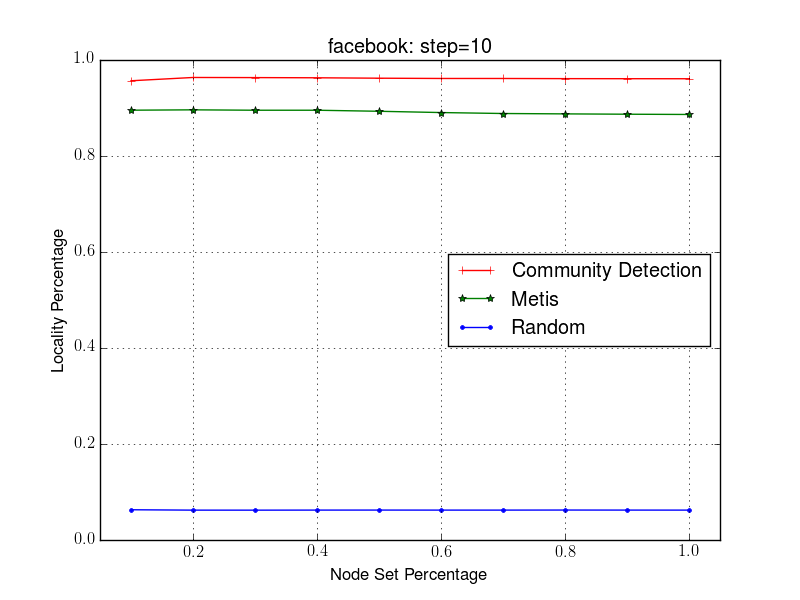
\includegraphics[width=0.45\columnwidth]{facebook_exp1.png}}
  \hfill
  \subfigure[Bar Chart]{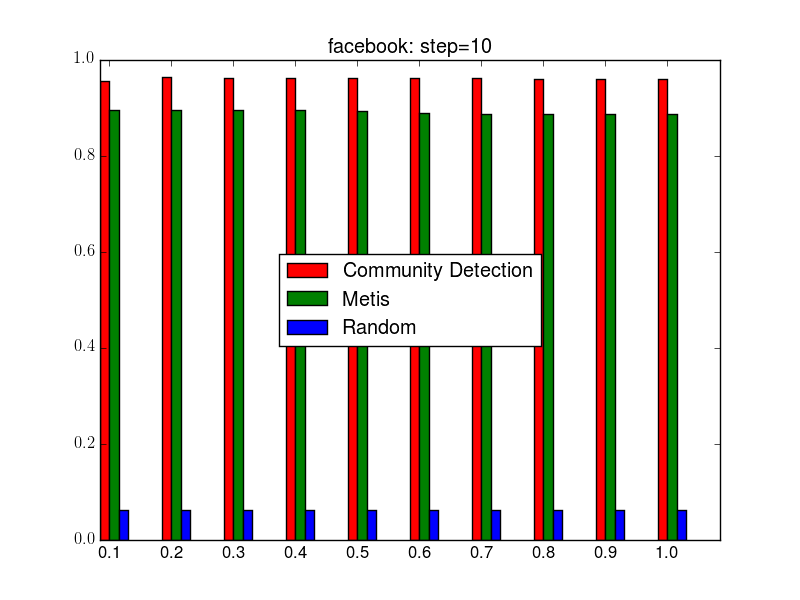
\includegraphics[width=0.45\columnwidth]{facebook_exp1_bar.png}}
  \hfill
  \caption{Facebook Locality}\label{fig:exp1_facebook}
\end{figure}

\begin{figure}[t]
  \centering
  \hfill
  \subfigure[Line Chart]{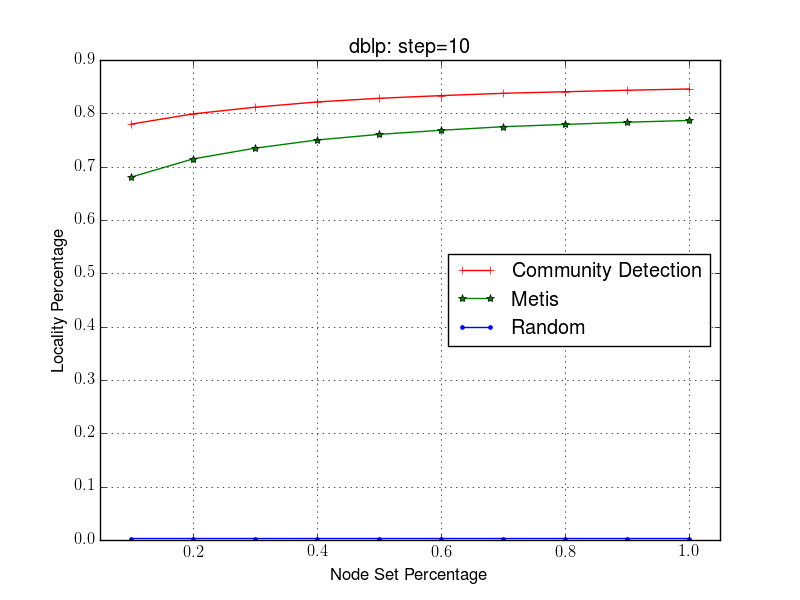
\includegraphics[width=0.45\columnwidth]{dblp_exp1.png}}
  \hfill
  \subfigure[Bar Chart]{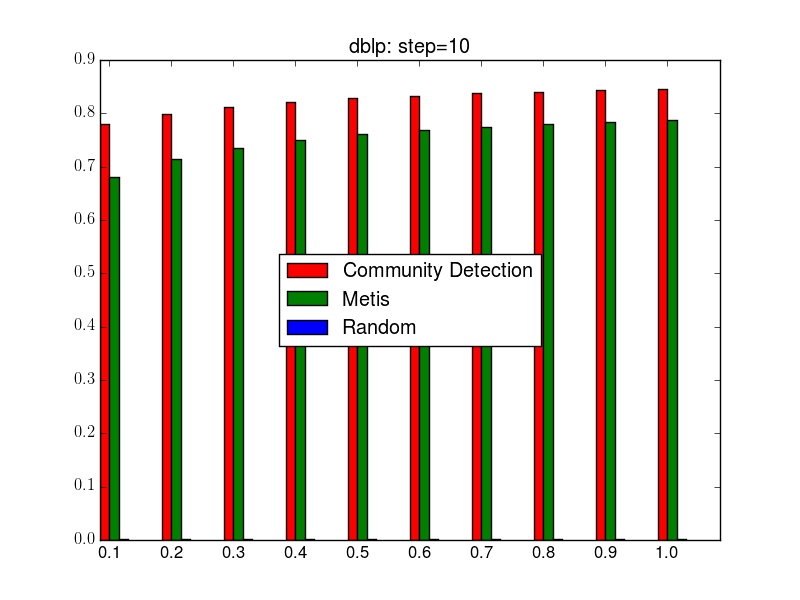
\includegraphics[width=0.45\columnwidth]{dblp_exp1_bar.png}}
  \hfill
  \caption{Facebook Locality}\label{fig:exp1_dblp}
\end{figure}

From Figure \ref{fig:exp1_facebook} it is obvious that the random partition approach has the lowest average locality, the value is around $6\%$, while the other two have approimated $90\%$. It is also interesting to notice that those nodes that have more neighbors have a greater impact on the locality.

\subsection{The Separated Parts Impact on Locality}

\begin{figure}[t]
  \hfill
  \subfigure[facebook]{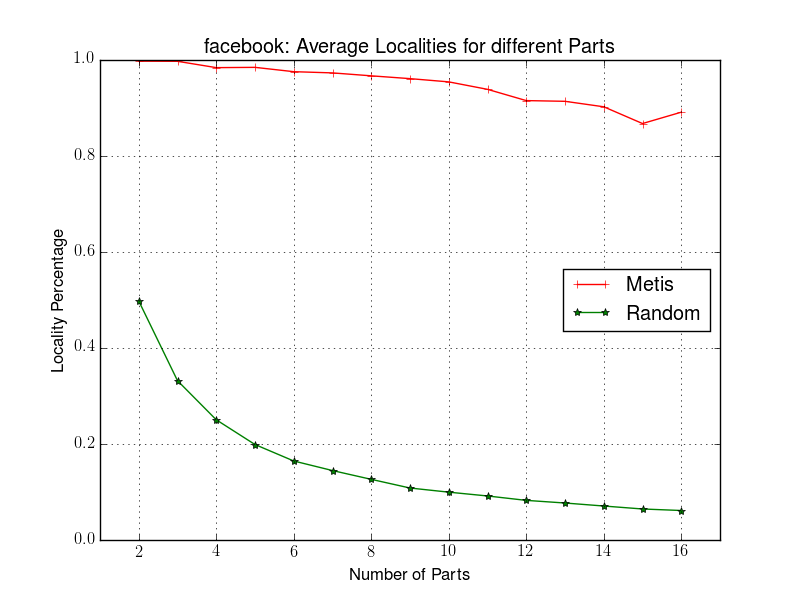
\includegraphics[width=0.45\columnwidth]{facebook_exp2.png}}
  \hfill
  \subfigure[dblp]{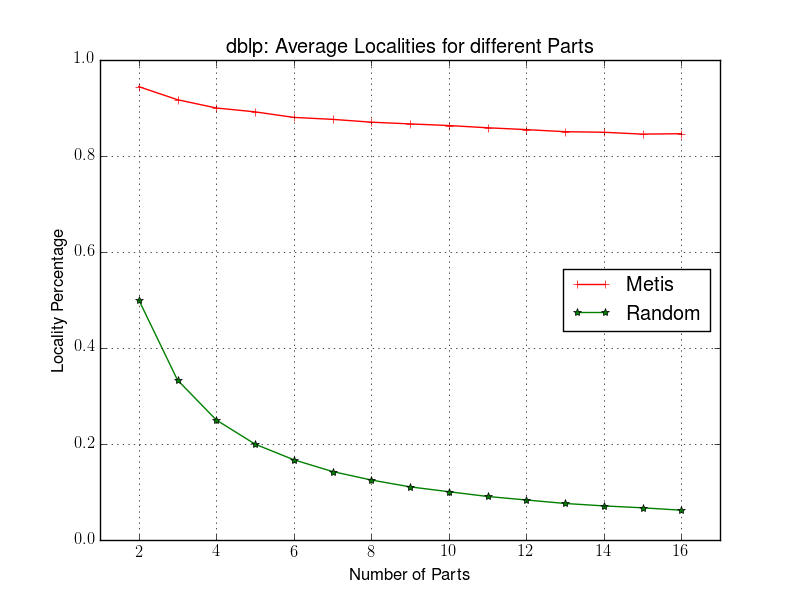
\includegraphics[width=0.45\columnwidth]{dblp_exp2.png}}
  \hfill
  \caption{Facebook Locality}\label{fig:exp2}
\end{figure}

\begin{figure}[t]
  \hfill
  \subfigure[facebook]{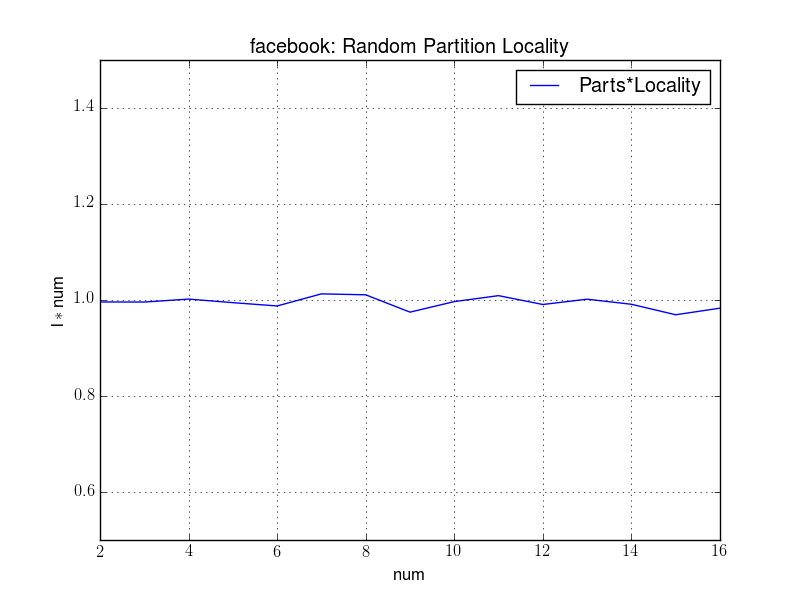
\includegraphics[width=0.45\columnwidth]{facebook_exp2_rnd.png}}
  \hfill
  \subfigure[dblp]{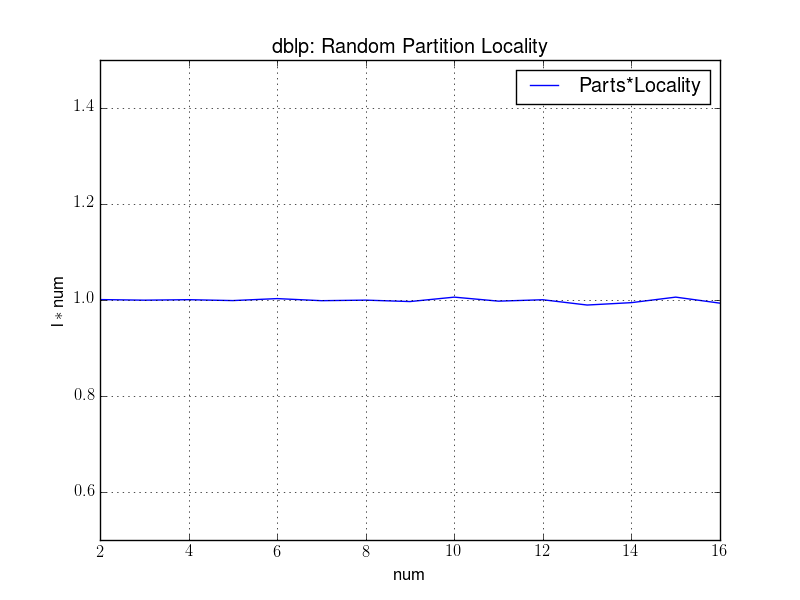
\includegraphics[width=0.45\columnwidth]{dblp_exp2_rnd.png}}
  \hfill
  \caption{Facebook Locality}\label{fig:exp2}
\end{figure}
